\section{Modellazione end-effector}
L'obiettivo di questo capito consiste nel presentare la modellazione della cinematica e dinamica dell'end-effector.
\\L'end-effector, denominato anche come utensile, è composto da due componenti, azionati da due motori, il primo componente è una vite a ricircolo di sfere, il secondo invece è una guida lineare. 
\begin{table}[h!]
\centering
\begin{tabular}{|c |c |c|} 
 \hline
 Nome & Descrizione  & Valore \\ [0.5ex] 
 \hline\hline
 $m_v [kg]$ & massa vite  & 0.36 \\ 
 $p_v [m]$ & passo vite & 0.02 \\
 $I_v [kg\cdot m^2]$ & momento inerzia vite  & $6.40\cdot 10^{-6}$ \\
 \hline
\end{tabular}
\caption{Parametri end-effector}
\label{table:2}
\end{table}
A livello teorico si è partito definendo una legge di modo per i due componenti dell'end-effector, per entrambi la legge è polinomiale, la differenza però sta nel fatto che per la guida la facciamo sulla posizione mentre per la vite sull'orientamento.
\subsection{Cinematica end-effector}
Come abbiamo anticipato nell'introduzione di questa sezione abbiamo la presenza di due leggi di moto che andiamo a chiamare $z_ee$ e $\varphi_v$. Da queste condizioni iniziali dobbiamo ricavare la cinematica di posizione, andiamo quindi ad introdurre la Jacobiana dell'end-effector in questo modo: 
\begin{equation*}
J_e =
    \begin{bmatrix}
    \frac{p_v}{2\cdot \pi} & \frac{p_v}{2\cdot \pi} \\
    0 & 1
    \end{bmatrix}
\end{equation*}
Andiamo ora ad introdurre la variabile V con le sue rispettive derivate, che saranno i risultati della cinematica diretta di posizione, velocità ed accelerazione:
\begin{equation*}
    V = 
    \begin{bmatrix}
     Z \\ 
     \theta_Z
    \end{bmatrix}, 
    \dot{V} = 
    \begin{bmatrix}
    \dot{Z} \\ \dot{\theta_Z}
    \end{bmatrix},
    \ddot{V} =
    \begin{bmatrix}
    \ddot{Z} \\ \ddot{\theta_Z}
    \end{bmatrix}
\end{equation*}
Per concludere andiamo ad eseguire le operazione di cinematica diretta in questo modo:
\begin{equation}
    V = J_e\cdot \begin{bmatrix}
    z_{ee} \\ \varphi_v
    \end{bmatrix},
    \dot{V} = J_e\cdot \begin{bmatrix}
    \dot{z_{ee}} \\ \dot{\varphi_v}
    \end{bmatrix},
    \ddot{V} = J_e\cdot \begin{bmatrix}
    \ddot{z_{ee}} \\ \ddot{\varphi_v}
    \end{bmatrix}
\end{equation}

\subsection{Dinamica della vite}
Per la definizione della dinamica della vite come tecnica è stata usata quella del PLV, come è stato fatto anche per la modellazione della dinamica dei bracci. 
\begin{equation*}
    inserire equazione?
\end{equation*}
Da questa si nota che abbiamo bisogno delle accelerazioni dei due elementi, andando a sviluppare i calcoli otteniamo la coppia come segue:
\begin{equation}
    C_ee = \begin{bmatrix}
    m_e & 0 \\ 0 & I_v
    \end{bmatrix}
    \cdot J_e\cdot \begin{bmatrix}
    \ddot{z_{ee}} \\ \ddot{\varphi_v}
    \end{bmatrix}
\end{equation}
Nella seguente immagine è possibile vedere il risultato di questo calcolo, con ingresso la legge di moto polinomiale
\begin{figure}[ht]
\begin{center}
    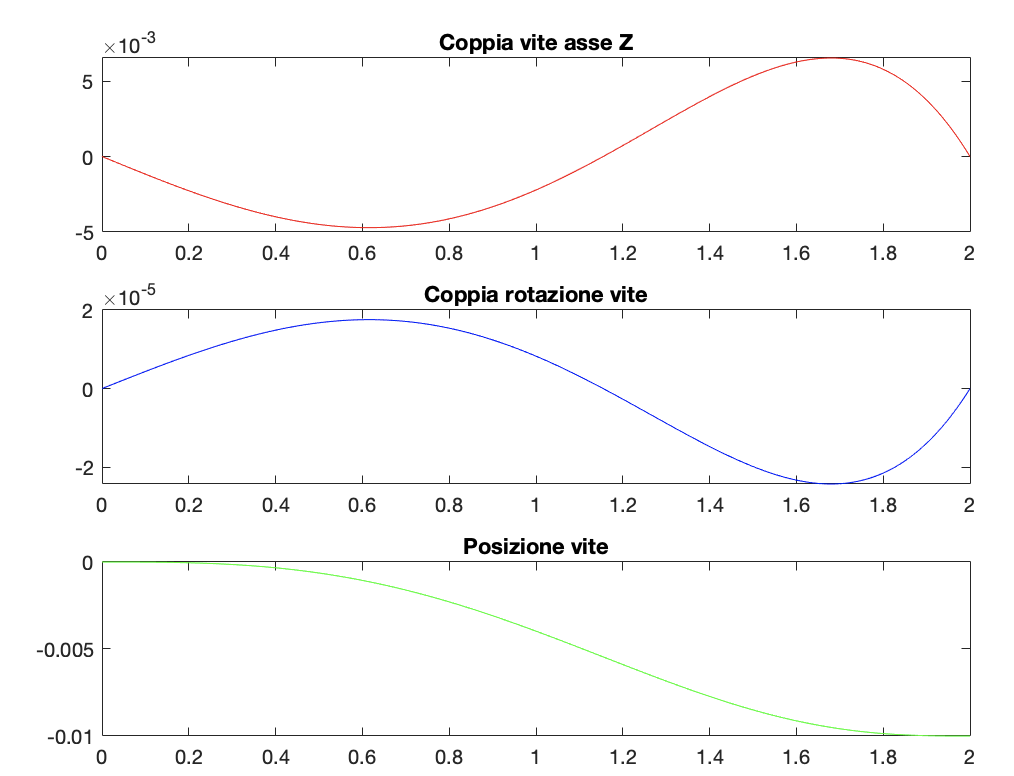
\includegraphics[scale=0.55]{Immagini/coppiaTeoricaVite.png}
    \caption{Coppie e posizione end-effector}
\end{center}
\end{figure}
In particolare sono mostrate le coppie dei due componenti e la posizione finale dell'end-effector
\subsection{Modellazione su Adams}